\section{Simulation Analysis}
\label{sec:simulation}

\paragraph{} In this section we analised the circuit making use of the NGSpice software. Given that this circuit has a sinusoidal voltage source, the current that flows trough the circuit components varies with time.
As such, in order to simulate the circuit's total response we must run a transient analysis. We also ran an operating point analysis for $t < 0$ and $t = 0$.

\subsection{Operating Point Analysis}

Below we can find the simulated operating point results for  $t < 0$ and $t = 0$:

[INSERIR TABELAS]

For $t<0$ we replaced the capacitor with a voltage source $V_x$ in order to determine the equivalent resistor.

[INSERIR CÁLCULO DA Req]

\subsection{Natural Response}

The graphic bellow is the plot of $v_6(t)$ for the $[0, 20]ms$ time interval, using transient analysis simulation.

\begin{figure}[!h]
	\centering
	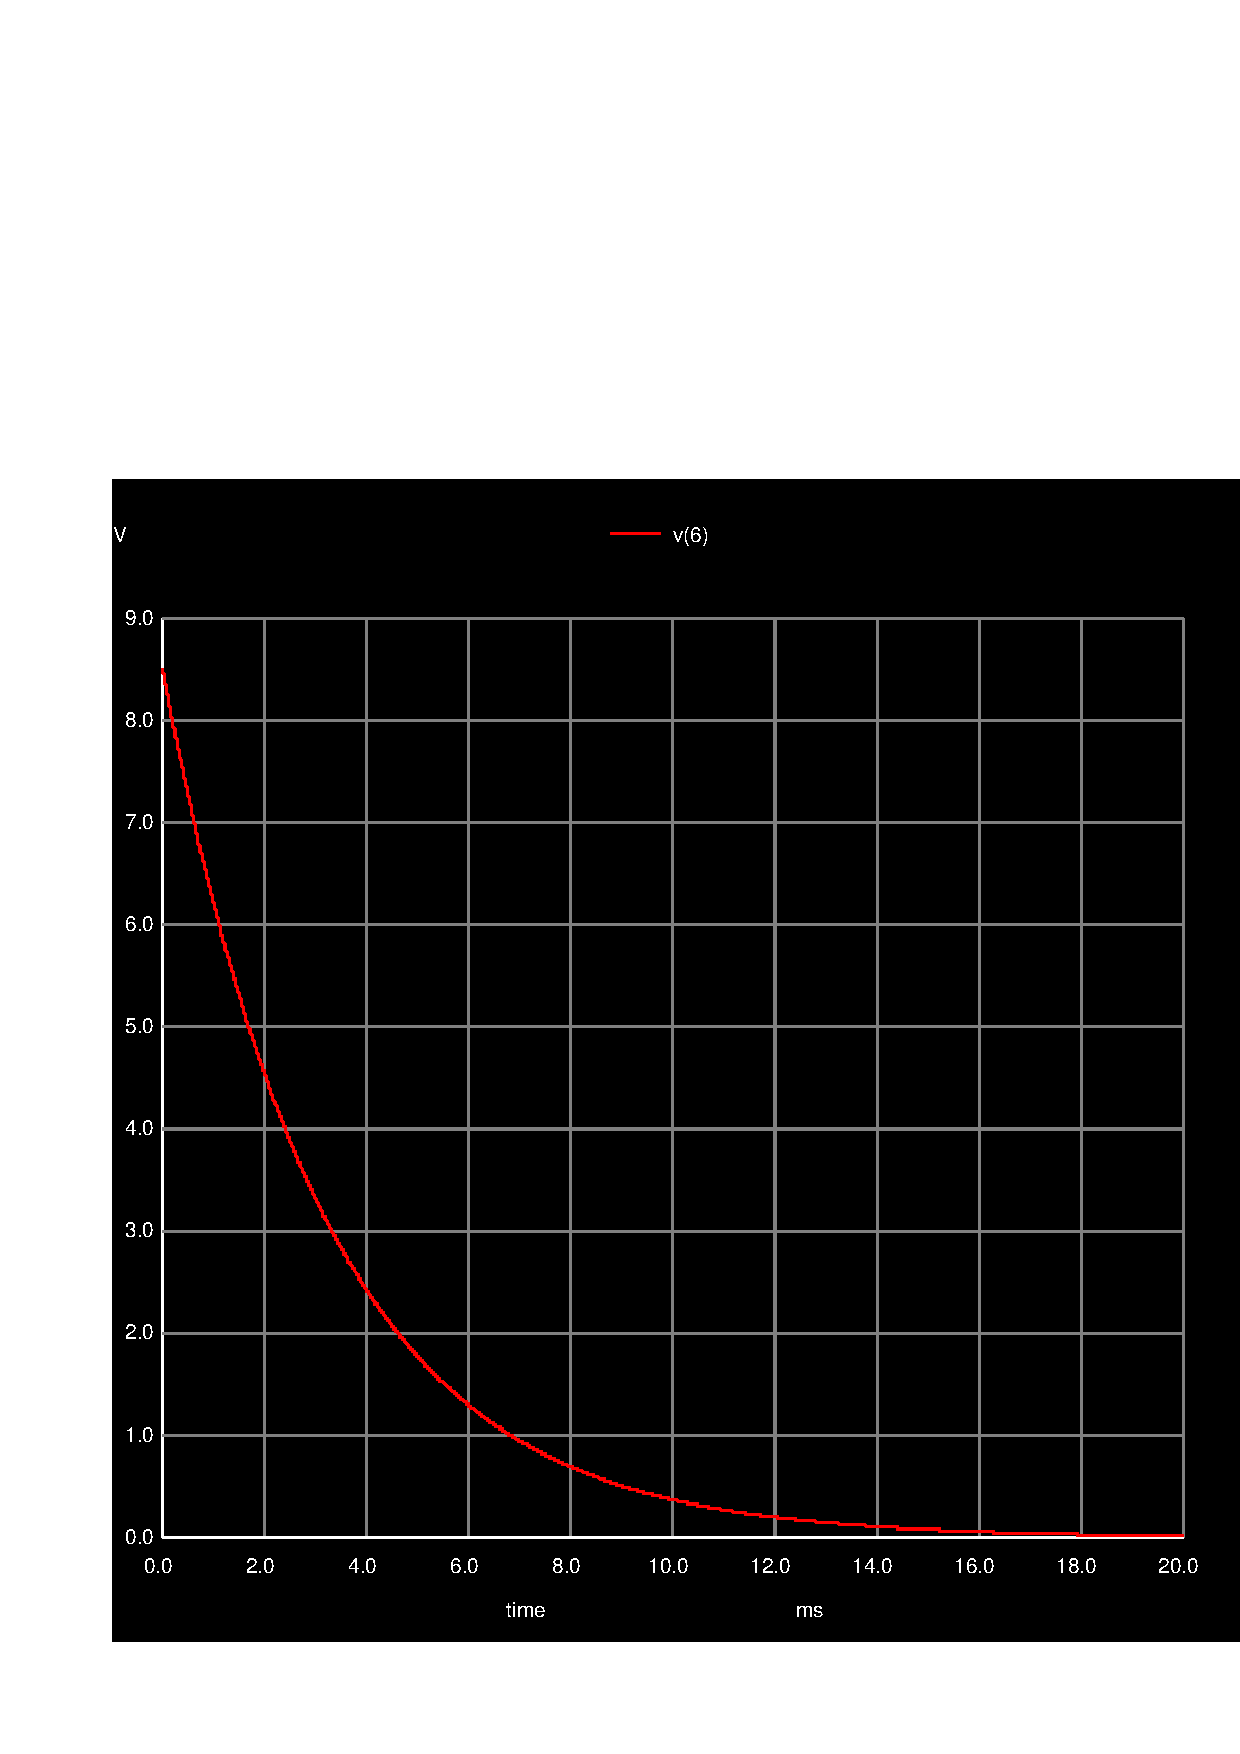
\includegraphics[width=0.7\linewidth]{../sim/natural.pdf}
	\caption{Natural response simulated for the $V_6$ voltage}
\end{figure}

\subsection{Total Response}

The previous step was repeated, this time considering $v_s(t)$ and f = 1kHz. In the plot below we have both the stimulus and the response.

\begin{figure}[!h]
	\centering
	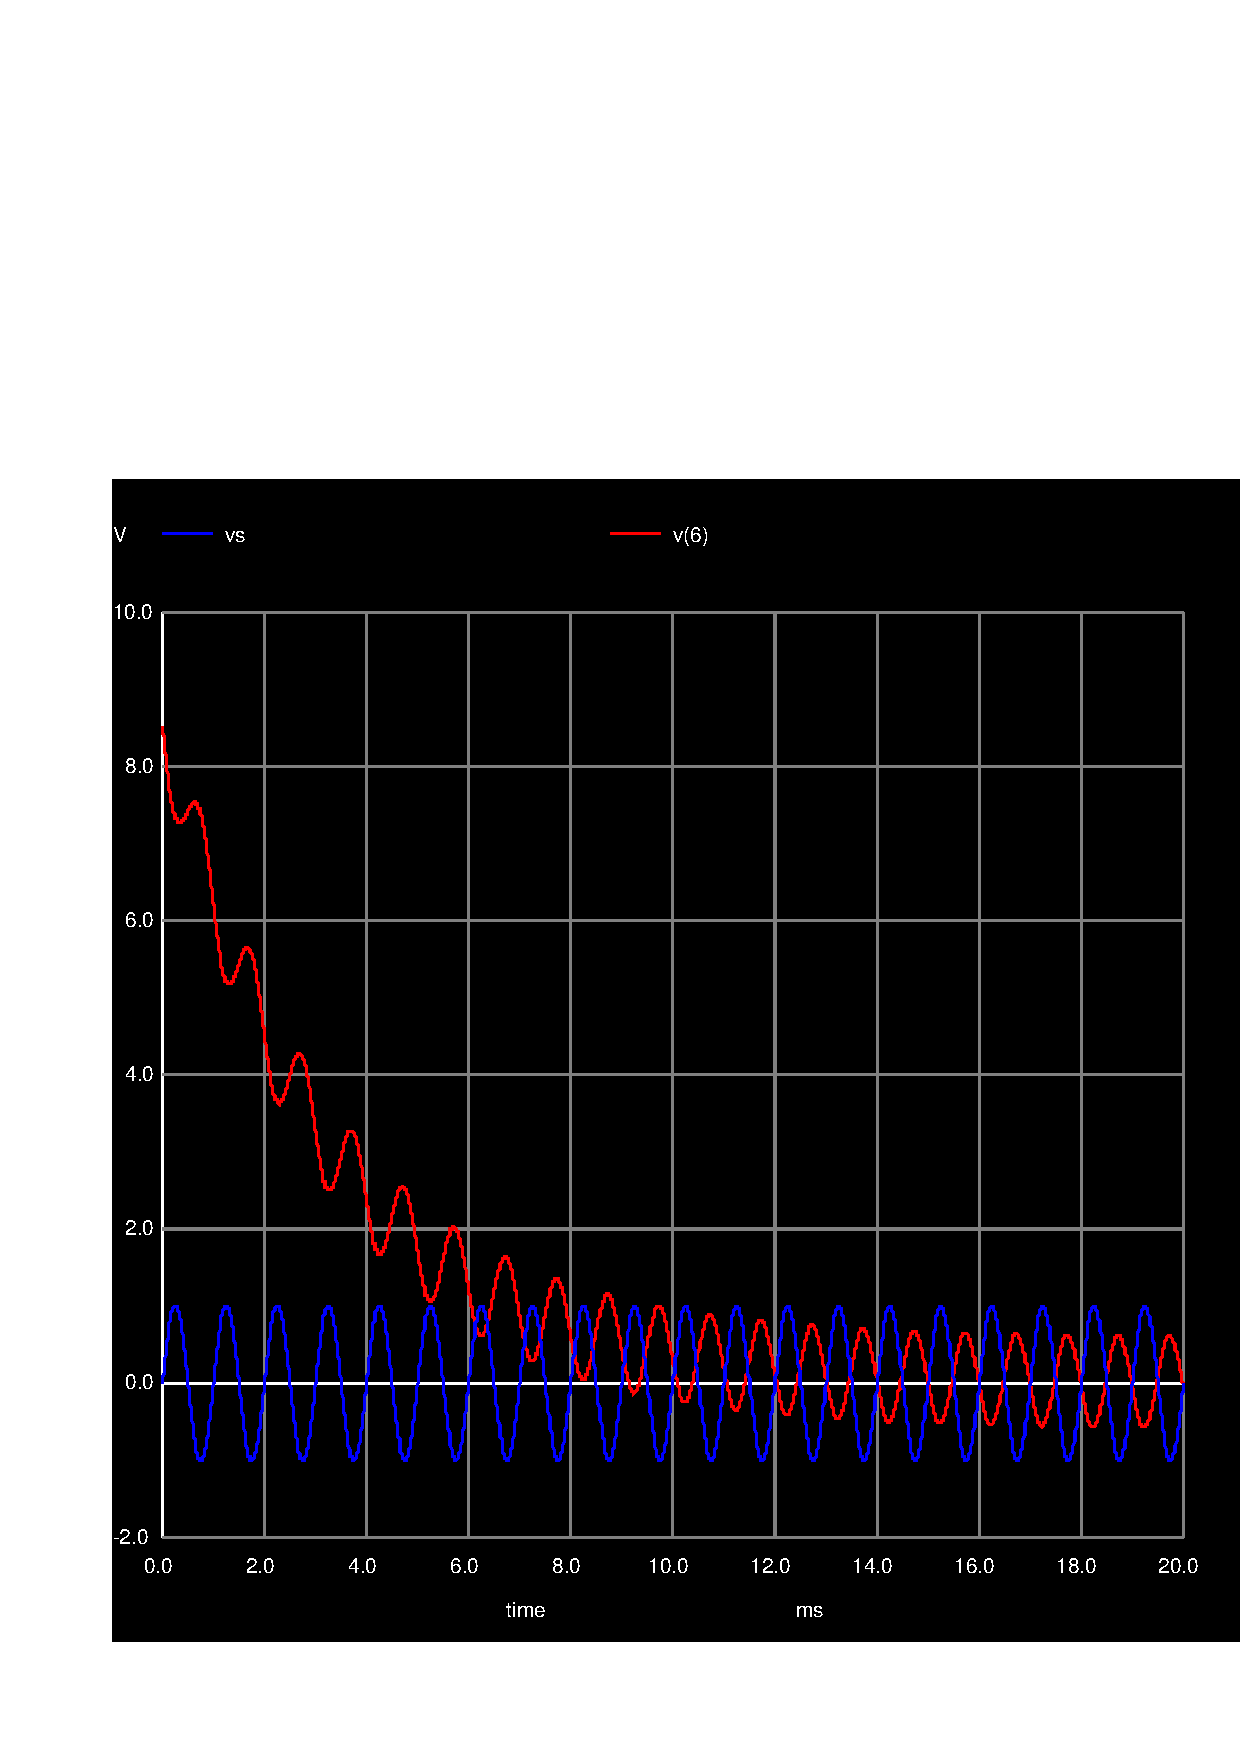
\includegraphics[width=0.7\linewidth]{../sim/total.pdf}
	\caption{$V_6$ and $V_S$ voltages simulated responses}
\end{figure}


\subsection{Frequency Response}

Analogous to the theoretical analysis we can find bellow:

\begin{figure}[!h]
	\centering
	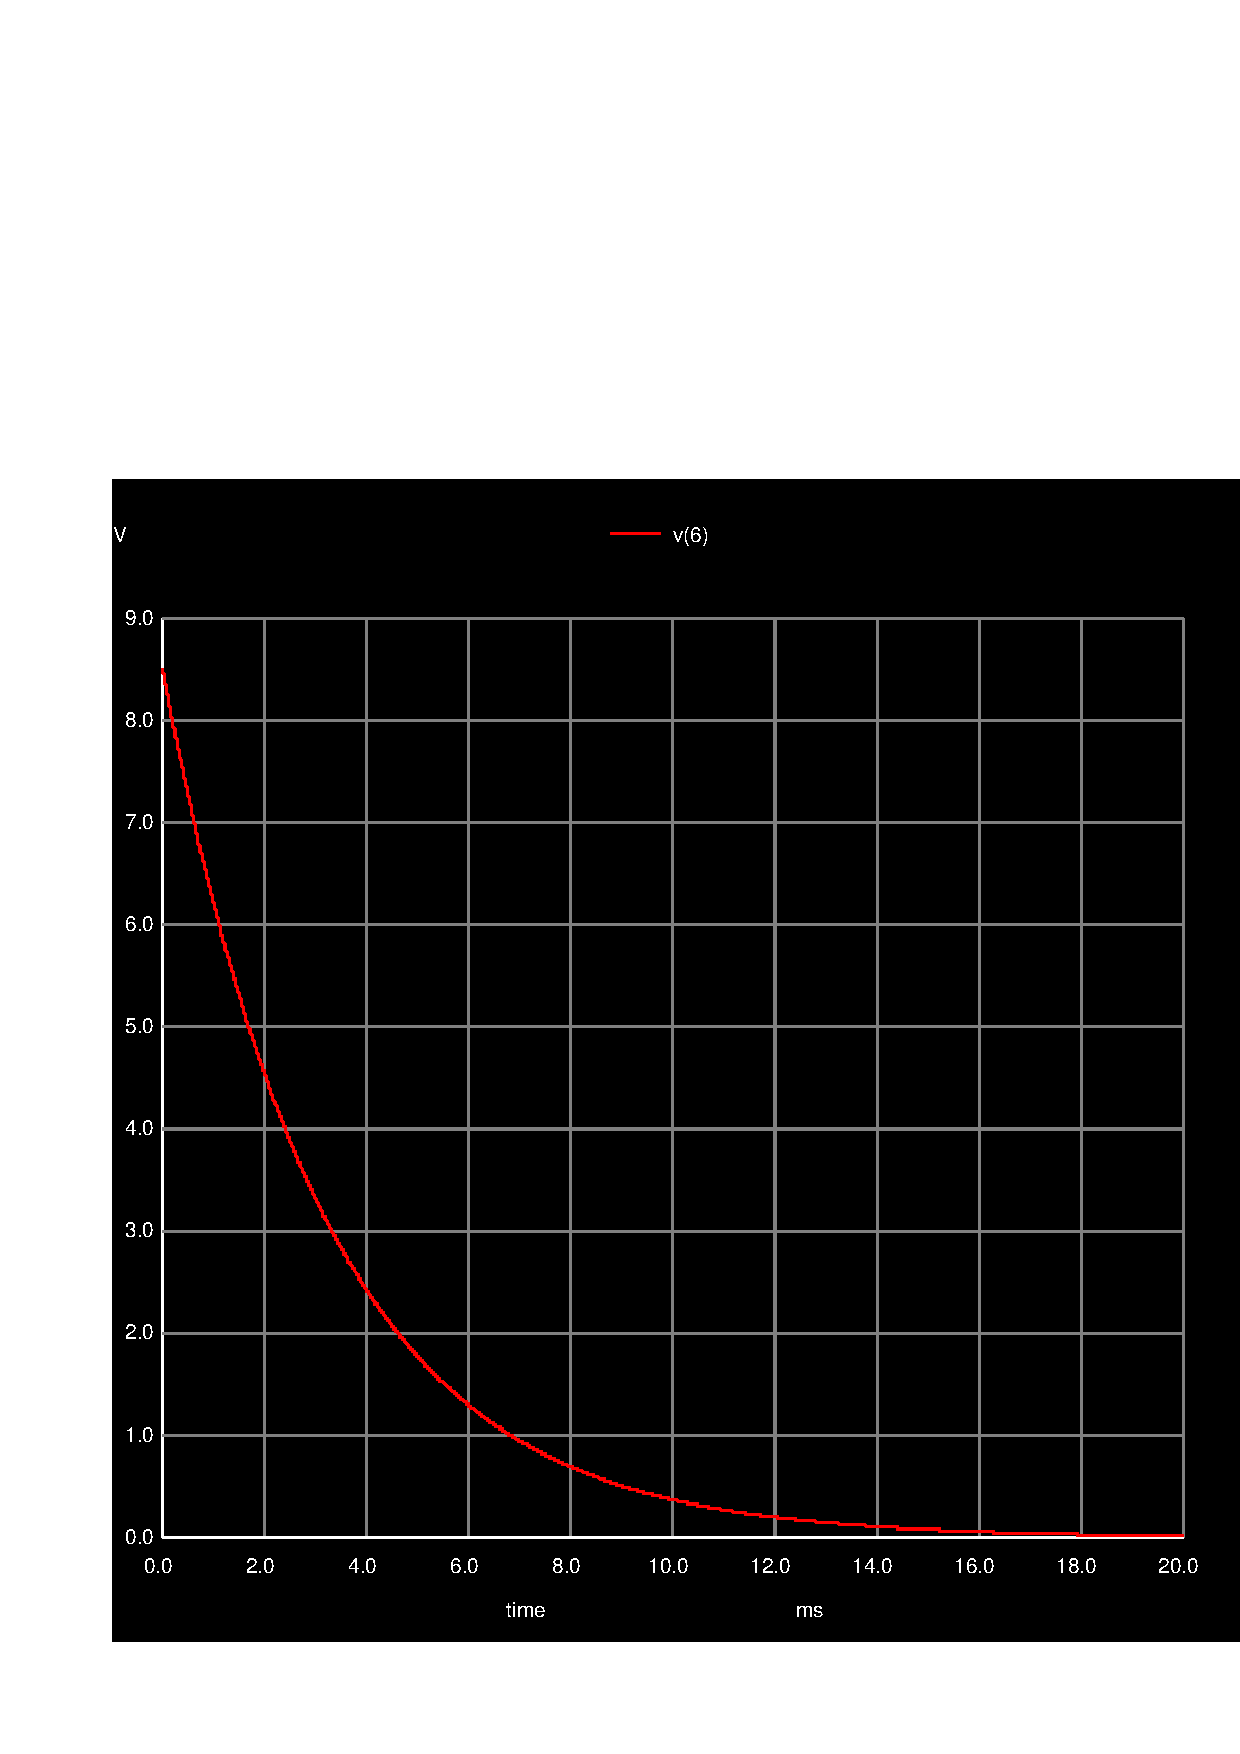
\includegraphics[width=0.7\linewidth]{../sim/natural.pdf}
	\caption{Magnitude of $V_S$, $V_c$ and $V_6$ in function of frequency}
\end{figure}

\begin{figure}[!h]
	\centering
	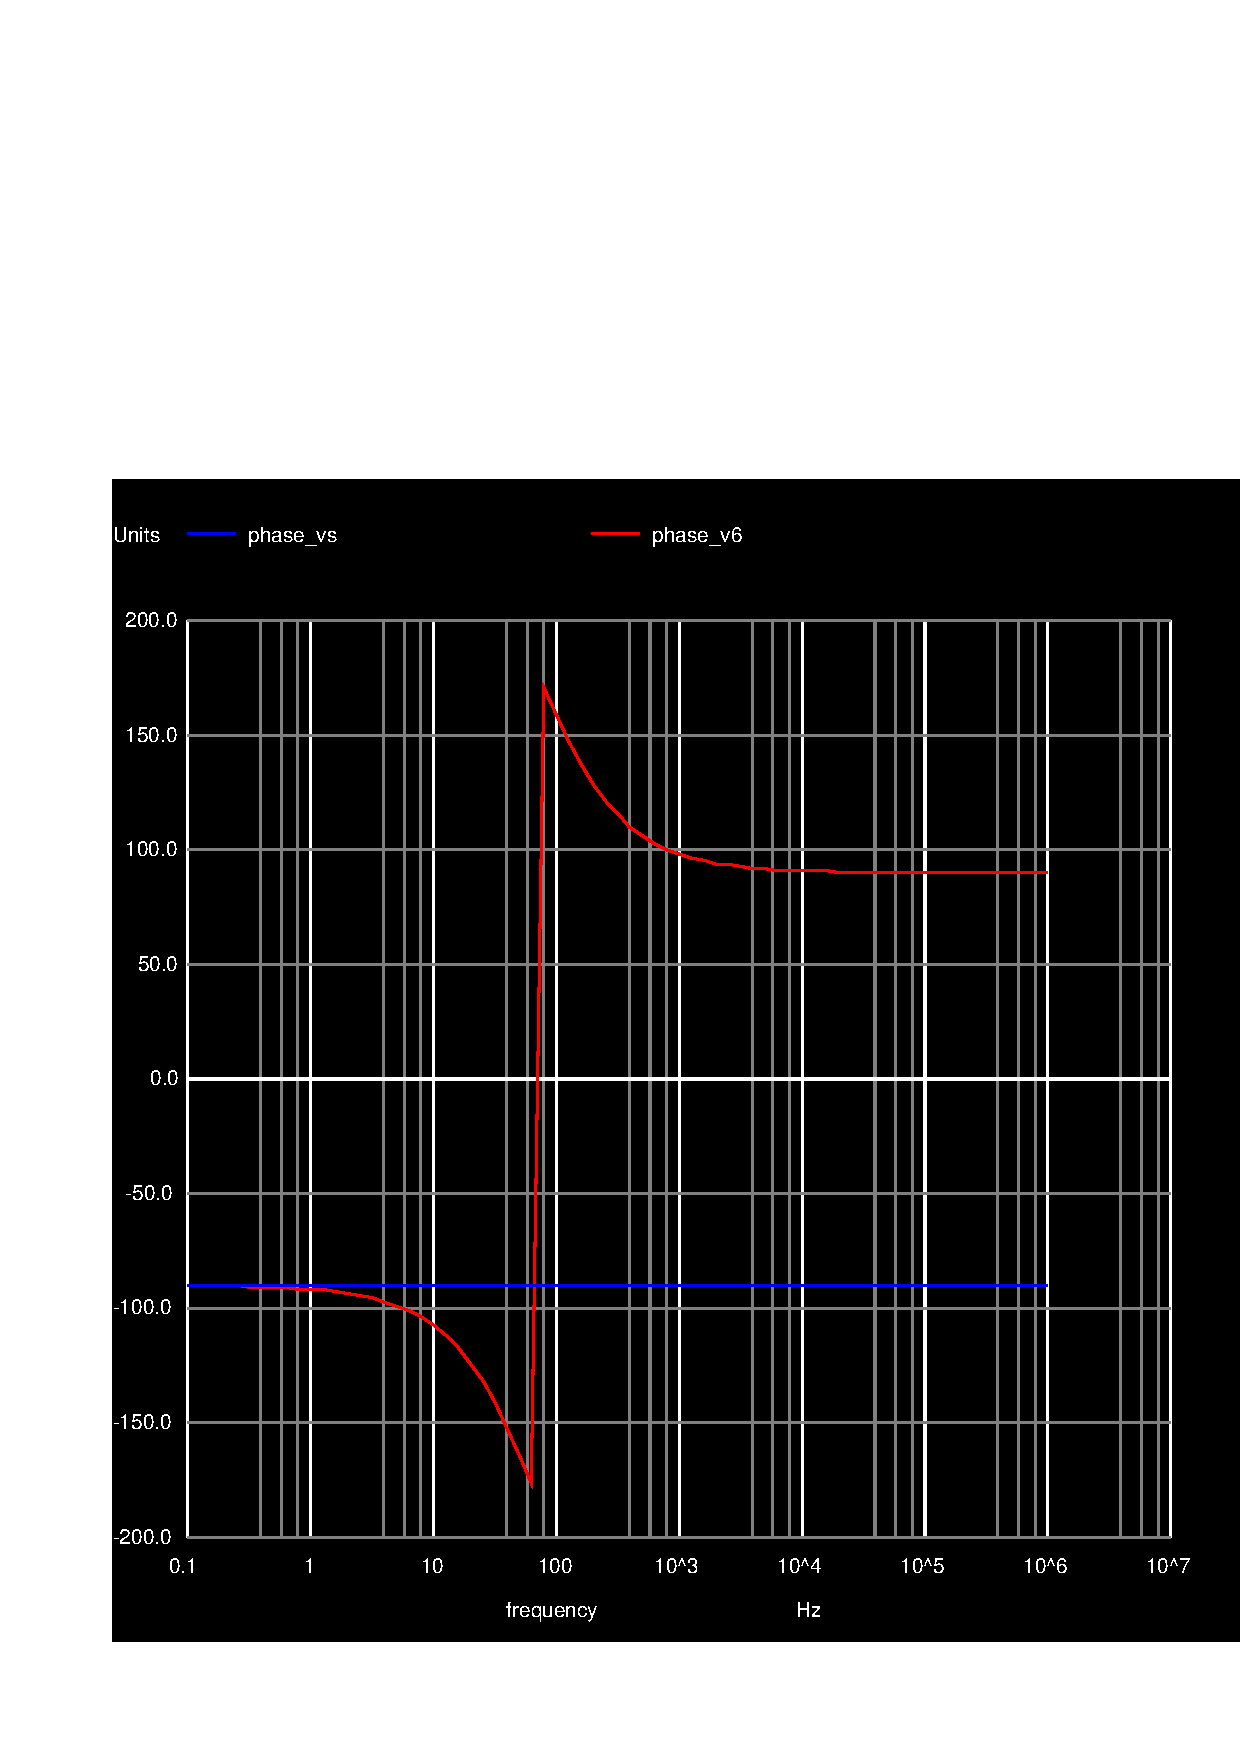
\includegraphics[width=0.7\linewidth]{../sim/phase.pdf}
	\caption{Phase of $V_S$, $V_c$ and $V_6$ in function of frequency}
\end{figure}